\documentclass{ecnreport}
\usepackage[export]{adjustbox}

\setlength{\parindent}{0cm}

\stud{Control \& Robotics master}
\topic{Mobile Robots}

\def\maze{\texttt{ecn::Maze}~}

\begin{document}

\inserttitle{Mobile Robots lab}

\insertsubtitle{Robot Control}


\section{Content of this lab and expected work}

The goal of this lab is to control a 2D mobile robot in order to follow a trajectory. Two mobile robots will be considered:
\begin{itemize}
 \item A 2-0 or unicycle robot, with two actuated, fixed wheels.
 \item A 1-1 or bicycle-like robot, with two passive fixed wheels and an actuated, steering wheel.
\end{itemize}

Two control laws will be tested for each robot: static feedback and Lyapunov-based control.\\

In addition, robustness of the control will be analyzed with regards to several practical issues:
\begin{itemize}
 \item Bad calibration, ie wrong dimensions of the robot model 
 \item Non linearities, which are typically found with saturation on wheel velocities or angles.
\end{itemize}

The control laws will be tested in simulation with Matlab/Simulink.\\
Trajectory generation is partially given and we assume a localization method is here and provides the current posture $(x,y,\theta)$  of the robot. 

\section{Available tools}

Two folders are available in the Matlab workspace, called \texttt{2-0} and \texttt{1-1}.
Each folder contains a Matlab script file and a Simulink model. The figure below shows the 2-0 model:
\begin{figure}[h]\centering
 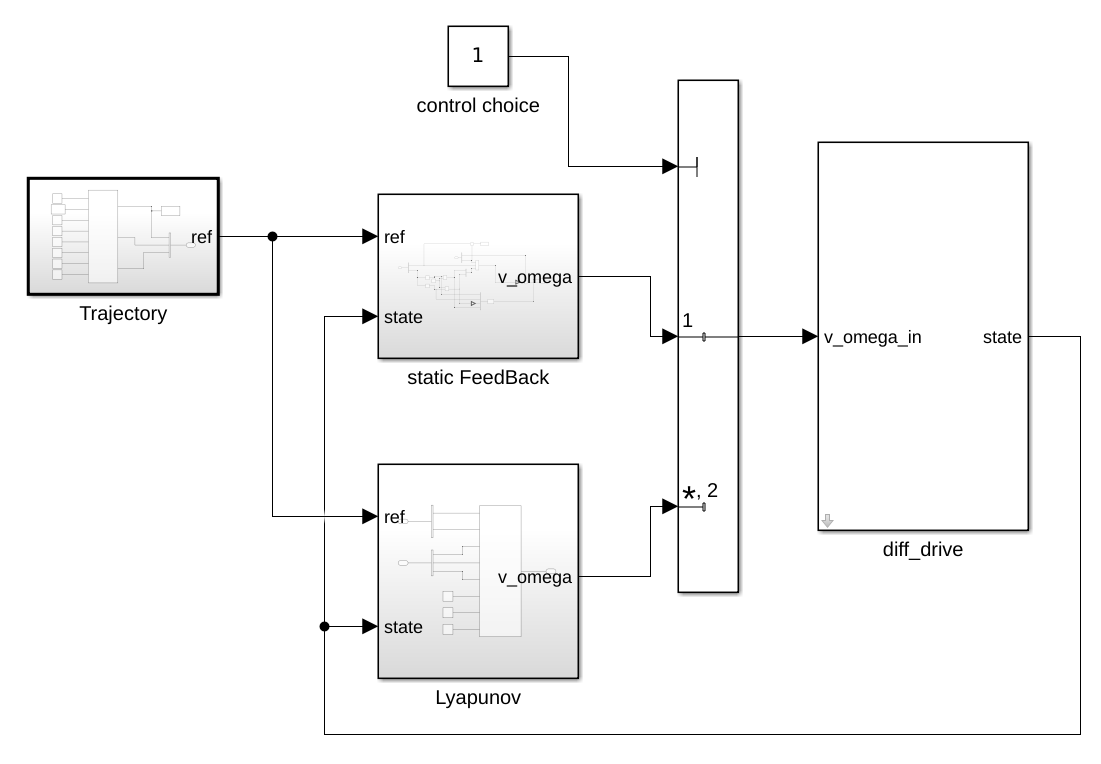
\includegraphics[width=.64\linewidth]{simulink}
\end{figure}

\newpage

Five main blocks appear:
\begin{itemize}
 \item \texttt{Trajectory}: Generates the trajectory. The \texttt{ref} output is a structure containing the desired position, velocity and acceleration.
 \item \texttt{diff\_drive}: The model of the robot, takes the control inputs and updates the state of the robot.
 \item \texttt{static FeedBack} / \texttt{Lyapunov}: Control blocks, take the reference and state and output the command.
 \item \texttt{Control law switch}: Allows to choose control depending on the value (1 or 2).
\end{itemize}

The given script will generate a trajectory from waypoints, then run the simulation and plot the behavior of the robot. The parts to be modified are:
\begin{itemize}
 \item The content of the two control blocks
 \item The parameters of the robot model, including saturation and uncertainty
 \item If needed, the waypoint coordinates used to generate the trajectory, in order to test simpler or more complex trajectories.
\end{itemize}

Signals going through the reference and state should be decomposed by using a \texttt{Bus Selector} to retrieve the actual values:
\begin{figure}[h]
\begin{minipage}[c]{0.32\linewidth}
\centering
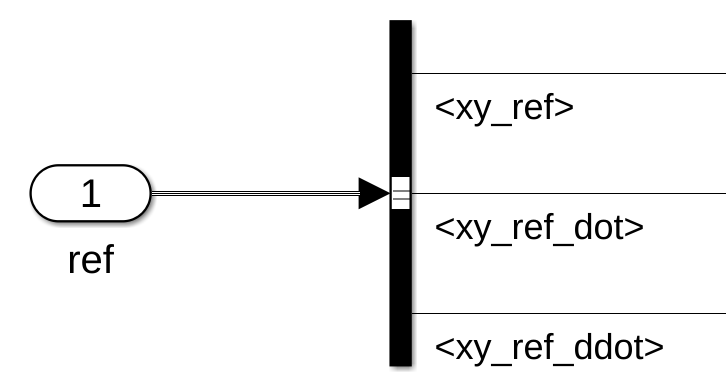
\includegraphics[height=0.4\linewidth, valign=c]{ref} \\ \footnotesize Reference to position, velocity and acceleration
\end{minipage}
\begin{minipage}[c]{0.32\linewidth}
\centering
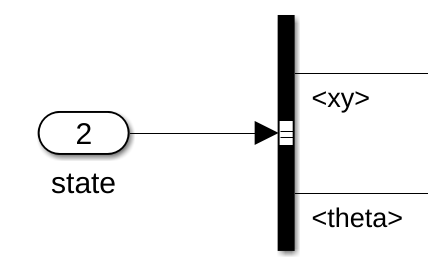
\includegraphics[height=0.4\linewidth, valign=c]{state20} \\ \footnotesize 2-0 robot state to $(x, y, \theta)$
\end{minipage}
\begin{minipage}[c]{0.32\linewidth}
\centering
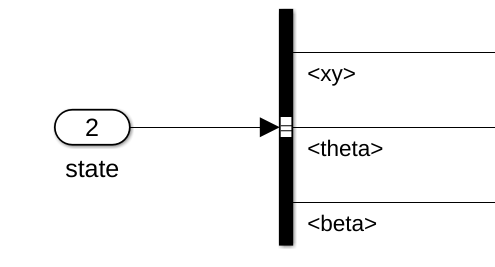
\includegraphics[height=0.4\linewidth, valign=c]{state11} \\ \footnotesize 1-1 robot state to $(x,y,\theta,\beta)$
\end{minipage}
\end{figure}

\paragraph{Trajectory generation} Initially the trajectory is always $(0,0)$ as shown in the next figure.
\begin{center}
 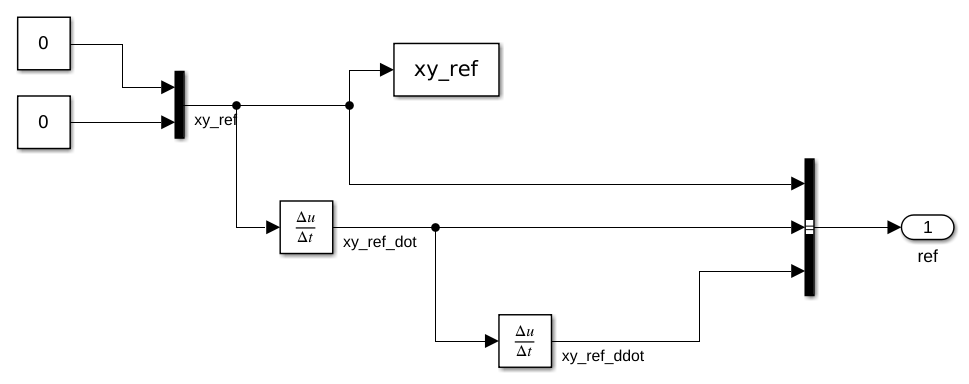
\includegraphics[width=.6\linewidth]{traj}
\end{center}
Two parameters $a$ and $w$ are defined in the initial script. They should be used to generate a circular trajectory:
\begin{center}
 $\left\{\begin{array}{ll}
          x(t) &= a\cos wt \\ y(t) &= a\sin wt \end{array}\right.$
\end{center}This trajectory will be followed during $t_{\max} = 2\pi/w$ which correspond to doing 3 turns.

\newpage

\section{Differential drive 2-0 robot}

The figure below recalls notations and kinematic model of a classical 2-0 mobile robot.

\begin{figure}[ht]
\begin{minipage}[t]{0.4\linewidth}
\centering
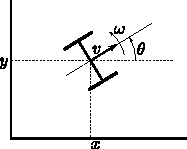
\includegraphics[%scale=1
                 width=0.8\linewidth, valign=c]{model20}
\end{minipage}%
\begin{minipage}[t]{0.6\linewidth}
{\renewcommand{\arraystretch}{1.2}
\begin{tabular}{ll}
 State & $(x, y, \theta)$ \\ 
 Parameters  & (base, radius) \\
 Control & $\u = (v, \omega)$ \\
 Kinematic model & 
 $ \left\{\begin{array}{l}
  \dot x = v \cos \theta \\
  \dot y = v \sin \theta \\
  \dot \theta =  \omega \\
 \end{array} \right.$
\end{tabular}}
\end{minipage}
\end{figure}

In practice the control input is mapped to wheel velocities through the base (wheel distance) and wheel radius parameters. The corresponding values can be changed by double-clicking the \texttt{diff\_drive} subsystem as shown in the figure below. Uncertainty on these parameters is initially set to 0.  \\

Non-linearity appears in the 2-0 model when we consider limitation on the wheel velocities. This parameter can also be tuned in the subsystem, it is initially set to a high value in order to reduce its impact.

\begin{figure}[ht]
\centering
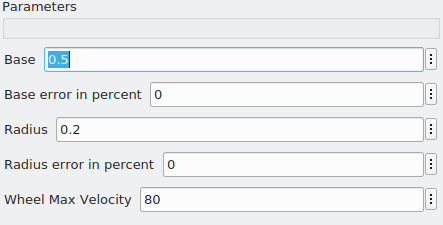
\includegraphics[width=0.4\linewidth]{param20}
\caption{Parameters for the differential drive robot}
\end{figure}

\subsection{Static feedback}

For static feedback, we want to control the position $\x_p = (x_p,y_p)$ of a point located at $d > 0$ on the x-axis of the robot.
It can be written as: 
\begin{center}
 $\left\{\begin{array}{ll}
         x_p &= x + d.\cos\theta \\
         y_p &= y + d.\sin\theta 
        \end{array}\right.$
\end{center}
The first step is to link $\dot \x_p$ to the control input: $\dot \x_p = \K(\theta).\u$.
\\

Then, a simple Proportional control is used to define the desired velocity of the point:
\begin{center}
$\dot \x_p^* = \dot \x_r + K_p(\x_r - \x_p)$
\end{center}
The final control law is thus:
\begin{center}
$\u = \K^{-1}(\theta) .\left(\dot \x_r + K_p(\x_r - \x_p)\right)$
\end{center}

Implement this control and test it for various values of $d$ and $K_p$. Once acceptable values have been found:
\begin{itemize}
 \item What happens when there are calibration errors?
 \item What happens when wheel rotation velocity is saturated?
\end{itemize} 

\subsection{Lyapunov-based control law}

In this approach, the goal is to minimize an energy function that should be equal to 0 when and only when the robot is at the target position and orientation. For 2-0 robots, a classical one is:
\def\W{\mathbf{W}}
\begin{center}
 $\W = \displaystyle \frac{1}{2}\left(x_e^2 + y_e^2 + \frac{\theta_e^2}{K_y}\right)$
\end{center}
where $(x_e, y_e, \theta_e)$ is the error in position and heading, corresponding to the target point expressed in the robot frame. They can be obtained easily from the reference values:
\begin{center}
 $\left\{\begin{array}{ll}
  x_e &= \cos\theta.(x_r-x) + \sin\theta.(y_r-y) \\
  y_e &= -\sin\theta.(x_r-x) + \cos\theta.(y_r-y) \\
  \theta_e &= \text{atan2}(\dot y_r, \dot x_r) - \theta \quad  \text{(put back in } [-\pi, \pi]\text{)}
\end{array}\right.$
\end{center}
A candidate control law is thus:
\begin{center}
 $\left\{\begin{array}{ll}
          v &= v_r\cos\theta_e + K_x x_e \\
          \omega &= \displaystyle\omega_r + K_y y_e v_r \frac{\sin\theta_e}{\theta_e} + K_\theta \theta_e
         \end{array}\right.$
\end{center}
Where $v_r$ and $\omega_r$ are feedforward control inputs, that can be obtained by:
\begin{center}
 $\left\{\begin{array}{ll} 
          v_r &= \dot x_r\cos\theta + \dot y_r \sin\theta \\
          \omega_r &= \displaystyle\frac{\dot x_r \ddot y_r - \ddot x_r \dot y_r}{v_r^2}\quad  \text{(or 0 if } v_r = 0\text{)}
         \end{array}\right.$
\end{center}
Show that this control makes $\W$ a Lyapunov function, meaning that its derivative is always negative except when the error is null.\\

Implement this control and test it for various values of $(K_x, K_y, K_\theta)$. Once acceptable values have been found:
\begin{itemize}
 \item What happens when there are calibration errors?
 \item What happens when wheel rotation velocity is saturated?
\end{itemize} 

\newpage

\section{Bicycle-like 1-1 robot}

The figure below recalls notations and kinematic model of a 1-1 mobile robot. Note that is also models classical cars as the two steering wheels angles are linked to a single, virtual centered wheel angle.

\begin{figure}[ht]
\begin{minipage}[t]{0.4\linewidth}
\centering
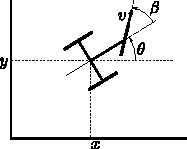
\includegraphics[%scale=1
                 width=0.8\linewidth, valign=c]{model11}
\end{minipage}%
\begin{minipage}[t]{0.6\linewidth}
{\renewcommand{\arraystretch}{1.2}
\begin{tabular}{ll}
 State & $(x, y, \theta, \beta)$ \\ 
 Parameters  & (L, radius) \\
 Control & $\u = (v, \dot \beta)$ \\
 Kinematic model & 
 $ \left\{\begin{array}{l}
  \dot x = v \cos \theta\cos \beta \\
  \dot y = v \sin \theta \cos \beta\\
  \dot \theta =  v\sin\beta / L \\
  \dot \beta =  u_2
 \end{array} \right.$
\end{tabular}}
\end{minipage}
\end{figure}

In practice the control input $v$ is mapped to wheel velocity through the wheel radius. The corresponding values can be changed by double-clicking the \texttt{bicycle} subsystem as shown in the figure below. Uncertainty on these parameters is initially set to 0. The $L$ parameter is the distance between the origin of the robot (middle of rear axle) and the steering wheel.  \\

Non-linearities appear in the 1-1 model when we consider wheel rotation velocity limit (limits $v$) and the wheel orientation limit in terms of $\beta$ and $\dot \beta$. These parameter can also be tuned in the subsystem, it is initially set to a high value in order to reduce its impact.

\begin{figure}[ht]
\centering
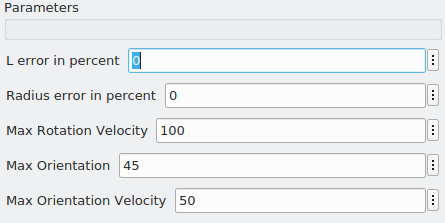
\includegraphics[width=0.4\linewidth]{param11}
\caption{Parameters for the bicycle-like robot}
\end{figure}

\subsection{Static feedback}

For static feedback, we want to control the position $\x_p = (x_p,y_p)$ of a point located at $d > 0$ in the direction of the steering wheel.
It can be written as: 
\begin{center}
 $\left\{\begin{array}{ll}
         x_p &= x + L.\cos\theta + d.\cos(\theta+\beta) \\
         y_p &= y + L.\sin\theta  + d.\sin(\theta+\beta)
        \end{array}\right.$
\end{center}
Follow the same approach as before to get the matrix $\K(\theta, \beta)$ such that: $\dot \x_p = \K(\theta, \beta).\u$.
\\

The same Proportional control can then be used to track the trajectory:
\begin{center}
$\u = \K^{-1}(\theta, \beta) .\left(\dot \x_r + K_p(\x_r - \x_p)\right)$
\end{center}

Implement this control and test it for various values of $d$ and $K_p$. Once acceptable values have been found:
\begin{itemize}
 \item What happens when there are calibration errors?
 \item What happens when wheel rotation velocity or wheel orientation is saturated?
\end{itemize} 

\subsection{Lyapunov-based control law}

The energy function in this case has the same form as in the 2-0 robot. It corresponds to the target position in the steering wheel frame, that can be written as:
\begin{center}
 $\left\{\begin{array}{ll}
  x_e &= \cos\theta.(x_r-x-L\cos\theta) + \sin\theta.(y_r-y-L\sin\theta) \\
  y_e &= -\sin\theta.(x_r-x-L\cos\theta) + \cos\theta.(y_r-y-L\sin\theta) \\
  \theta_e &= \text{atan2}(\dot y_r, \dot x_r) - \theta - \beta \quad  \text{(put back in } [-\pi, \pi]\text{)}
\end{array}\right.$
\end{center}
The control law is the same as before, but the $\omega$ component has to be mapped to the $\dot\beta$ control input with:
\begin{center}
 $\displaystyle \dot\beta = \omega - \frac{v}{L}\sin\beta$
\end{center}
Show that this control makes $\W$ a Lyapunov function.\\

Implement this control and test it for various values of $(K_x, K_y, K_\theta)$. Once acceptable values have been found:
\begin{itemize}
 \item What happens when there are calibration errors?
 \item What happens when wheel rotation velocity or wheel orientation is saturated?
\end{itemize} 





\end{document}
